\chapter{Fundamento Teórico}

Entendemos al proyecto gr-isdbt-tx como un complemento al trabajo de maestría presentado por Pablo Flores, por lo que nos parece reiterativo explicar en sumo detalle algunos de los fundamentos de telecomunicaciones sobre los que se construye la norma ISDB-T. Los mismos ya fueron explicados con gran claridad y nivel de detalle en la documentación de aquel proyecto. Quizás algunos de los lectores encuentren insuficiente el desarrollo de algunos de los conceptos incluidos en este capitulo. A ellos los invitamos a complementar la lectura de esta documentación con la tesis de maestría de Pablo Flores.

Es posible también que entre los lectores se encuentren técnicos vinculados al área de sistemas y programación.  Encontraran ellos, seguramente, mayor interés y profundidad de conceptos en los capítulos 4 y 5, donde detallamos el uso de GNU Radio como plataforma de SDR, y la estructura funcional de nuestro transmisor, así como los desafíos de programación a los que nos enfrentamos implementando cada uno de sus bloques. 

Intentando contemplar el interés de todos los lectores, es que les presentamos en este capitulo un repaso sobre algunos de los conceptos que entendemos clave para comprender por qué son necesarios algunos de los bloques del transmisor. 

Comenzaremos explicando aquí como se modela el canal inalámbrico para trabajar, que problemas se enfrenta uno cuando debe diseñar un sistema de transmisión por aire y como mitigar algunos de los efectos que el canal tendrá sobre nuestra señal. Repasaremos algunos de los códigos mas utilizados de detección y corrección de errores. Luego vendrá una breve explicación de los sistemas OFDM, su surgimiento teórico y práctico, para contextualizar algunas de las funcionalidades de ISDB-T. Para terminar, explicaremos de que forma se encapsulan los datos a transmitir. Para eso, repasamos algunos conceptos definidos en las normas MPEG, orientados hacia la transmisión de televisión, que ayudarán a modelar la fuente de datos del sistema.  

\section{Modelado del canal}

Cuando una señal viaja a través del aire, sufrirá una serie de modificaciones a causa de muchos factores. El clima, el ruido generado por otras señales que también viajan por el mismo medio, los rebotes de la señal contra edificios, autos o cualquier objeto que se encuentre en el camino, son todos aspectos que modificarán la señal, y por lo que la señal recibida sera distinta de la transmitida. 

De forma teórica, se podrían plantear las ecuaciones de Maxwell, definir condiciones de borde que modelen de manera fiel los obstáculos en el camino y calcular en cada momento y en cada lugar del espacio, la atenuación que afectará nuestra señal. Pero el canal cambia constantemente, las diferentes señales que comparten el medio también están en constante transformación, y por lo tanto no sería ni practico, ni útil seguir un camino como este para comprender el canal, mucho menos basarse en él para robustecer a la señal frente a los atenuantes que surgirán. 

Es por eso que se realiza un modelado menos ambicioso del canal. Consideramos al medio como un objeto mas simple, casi ideal, y la mayoría de las fuentes de interferencia se modelan dentro de una función de probabilidad a la que entendemos como ``ruido", que induce errores en el receptor. Este modelo del canal podrá ser mas o menos complejo, dependerá del técnico qué se enfrente al problema decidir que herramientas incluir en función de los efectos que desea mitigar en su señal.
	
Consideraremos en este documento, tres modelos distintos de canal, que serán los modelos de Gauss, Rice y Rayleigh. El primero, se utiliza fuertemente para el cálculo de enlaces punto a punto. Por su parte, el modelo de Rice, es bueno para modelar los enlaces punto a multipunto, por lo tanto se utiliza ampliamente en el mundo del broadcasting. Finalmente el modelo de Rayleigh considera los efectos de la difracción y los ecos producidos por las múltiples trayectorias.

\begin{itemize}
	\item Canal de Gauss
	
El canal de Gauss es el modelo mas sencillo de canal que se trabaja. Se modela al canal como un sistema cuyo efecto sobre la señal transmitida es la adición de un ruido blanco aleatorio (modelado mediante una distribución de probabilidad Gaussiana). En particular, es el modelo que se utiliza para calcular los enlaces punto a punto con linea vista. Generalmente, también se presenta la hipótesis de que el resto de las interferencias del canal, pueden modelarse como un ruido aditivo Gaussiano.
	
	\item Canal de Rice

El modelo de canal de Rice considera que un receptor estará expuesto primero hacia un haz directo, en lo que puede ser una transmision por linea vista, pero también considera otras trayectorias, debidas a los rebotes del haz original con los distintos obstáculos del entorno. Estos rayos secundarios generalmente vendrán acompañados de un determinado delay, de dimensión considerable.

	\item Canal de Rayleigh

En ISDB-T la transmision en la capa A esta orientada a la recepción en dispositivos móviles. De estos temas hablaremos mas adelante en el capitulo 3, pero por el momento, presentar esta idea nos da pie a plantear un modelo distinto de canal, uno en el que el receptor se mueve. 

El canal de Rayleigh tiene en cuenta las atenuaciones que se producen por lo que se conoce como Difracción Combinada, esto es, señales que sortean obstáculos perdiendo mucha de su potencia inicial en el proceso. Este fenómeno es interesante, puesto que puede llegar a existir transmision, pese a que no haya linea vista. 

Este modelo de canal toma mucha relevancia en ISDB-T, no solo porque la mayoría de los televisores tienen antenas internas, sino que tenemos que modelar el canal para resolver el problema de la recepción móvil. Es posible robustecer a la señal de forma tal que un teléfono móvil pueda decodificar datos multimedia en alta definición y con poca latencia en todo momento, sin perder la continuidad del servicio. 

Existen una serie de estrategias, implementadas en la norma ISDB-T, orientadas a resolver estos mismos problemas.

	\item Canal como un Filtro
	
	Aca va lo del cana, y hay que poner un enganche para lo de OFDM
\end{itemize}

\section{Modulación OFDM}

En 1966, Chang presenta un método para lograr la multiplexion canales de datos a través de un medio de frecuencia acotada\cite{chang-ofdm}, que elimina los efectos de interferencia intersimbolica e intercanal. Implico un cambio importante en la teoría de telecomunicaciones de la época, pues hasta entonces, los resultados existentes tomaban como funciones modulantes ortogonales, señales limitadas en el tiempo, lo que implica grandes anchos de banda en frecuencia, y en los canales de banda acotada implementados en la practica se traducían en interferencias producto de los recortes en banda. 

En el paper, Chang postula la idea de una nueva clase de funciones modulantes acotadas en frecuencia, que ademas, permite modular de manera independiente amplitud y frecuencia. En ese momento se sentaban las bases de la modulacion OFDM (Orthogonal Frecuency-Division Multiplexing).

Uno de los mayores problemas de los sistemas FDM, era la incapacidad para escalar en cantidad de canales. La complejidad y el costo de construir los osciladores para la cantidad de portadoras necesarias, mantenían la brecha entre la teoría y la practica. 

La solución a estos problemas, llega cuando se logra programar computadoras capaces de procesar grandes cantidades de datos, mediante la implementación del algoritmo de “Fast Fourier Transform”. 

Weinstein y Ebert, resolvieron en \cite{discrete-ofdm} el problema de la escalabilidad de los sistemas OFDM, mediante la conjugacion de los mencionados avances tecnologicos, discretizando las señales a transmitir, y modulandolas por computadora, en lugar de usar los bancos de osciladores. 

Una señal multitonal, puede ser vista como la transformada de fourier de un tren de pulsos, y la demodulacion coherente a su vez puede entenderse como la aplicación en tiempo continuo de una transformada inversa de Fourier. Entonces, probaron que muestreando la señal de origen, y mediante la implementación de un modem sobre una computadora que ejecute el algoritmo de la transofrmada rápida de Fourier, se pueden obtener aproximaciones suficientemente cercanas a los de la señal original. 

En principio el resultado es válido para un sistema OFDM con N canales simultáneos, con portadoras separadas en frecuencia en distancias suficientemente cercanas, como para aproximar la respuesta al impulso del canal, como si fuese de modulo constante sobre cada uno de los N canales. 

Pero falta un paso mas, pues la hipótesis del comportamiento del canal constante, se aleja bastante de la realidad. Plantearon entonces un canal de respuesta al impulso lineal en frecuencia.

En estas condiciones, y atendiendo ademas que la señal discreta a transmitir solo “vive” en el ancho de banda de transmisión, consideraron a la señal a transmitir como una transformada de Fourier enventanada. Desarrollando estas ideas lograron probar que, si la ventana es plana en las frecuencias de interés, y se agregan “guardas” de seguridad a ambos lados de las portadoras activas, de modo que las colas del enventanado caigan de forma continua, (alejando el enventanado de la idealidad de las ventanas rectangulares) se logran condiciones para reducir la distorsión generada por la respuesta al impulso del canal, a efectos transitorios de dispersión rápida, y la señal en recepción sigue convergiendo a la señal transmitida.

\section{Estrategias para mitigar los efectos del canal}

	\subsection{C\'odigos de detecci\'on y correci\'on de errores}

La comunicación entre emisor y receptor puede modelarse mediante el proceso de la Figura \ref{diagrama_codificacion}. La situación es la siguiente, una fuente emisora envía mensajes $m$ (palabras fuente) al receptor a través de un canal de comunicación. El mensaje debe ser traducido a algún mensaje que el canal esté capacitado para enviar, estos mensajes se conocen como palabras código.

\begin{figure}[h!]
\centering
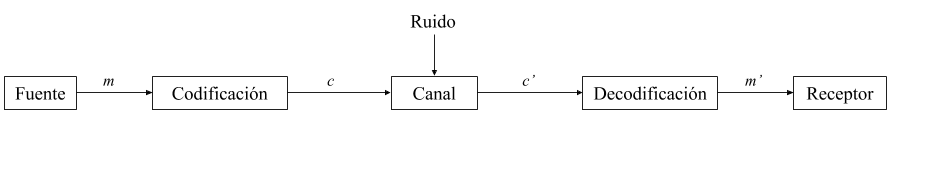
\includegraphics[scale=0.45]{figuras/cap02/diagrama_codificacion}
\caption{\label{diagrama_codificacion} Esquema básico de codificación de canal.}
\end{figure}

Al otro lado del canal llega un mensaje codificado $c'$, el cual seguramente sea erróneo, pues en todo proceso real de comunicación existe ruido e imperfecciones en los canales. El mensaje es decodificado en una palabra $m'$, y generalmente $m' \neq m$.

Se desea que el receptor sea capaz de darse cuenta si el mensaje $m'$ es realmente lo que se transmitió del otro lado, y más aún, poder corregirlo. 

La Teoría de Códigos es un campo de la matemática aplicada que busca resolver los problemas de las etapas de codificación-decodificación y corrección, y que presenta su propia complejidad.

La transmisión inalámbrica de una señal la expone a diversas fuentes de ruido, con lo cual los tipos de errores generados pueden ser muy variados. Por ejemplo los errores en ráfaga, en los que un conjunto de bits consecutivos se ven alterados, son muy comunes en las comunicaciones inalámbricas. También podría suceder que el canal radioeléctrico presente distorsión en algunas portadoras en particular.

El estándar ISDB-T hace uso de distintas técnicas para la protección de los datos en transmisión. De hecho para proteger los datos en los ejemplos mencionados el estándar utiliza las técnicas de \textit{entrelazamiento de bits y bytes} y la aplicación de códigos \textit{forward error correction} o FEC como es el caso de Reed Solomon. Para la comprensión del estándar y el desarrollo de \textit{gr-isdbt-tx}, es importante conocer el funcionamiento de estas técnicas. Profundizar en estos temas escapa los objetivos de este trabajo, por lo cual los detalles técnicos se pueden encontrar en las bibliografías mencionadas.

Para asegurarse que el receptor pueda llevar a cabo satisfactoriamente la demodulación y decodificación en una transmisión jerárquica, en la cual se utilizan múltiples parámetros de transmisión, se utiliza una señal denominada Transmission and Multiplexing Configuration Control (TMCC).

Como se verá en el Capítulo XX, la TMCC junto con otras señales piloto y las señales correspondientes a la transmisión de los datos útiles, conforman el cuadro OFDM.

Al tratarse de una señal que contiene información crítica sobre la transmisión se la debe proteger fuertemente frente a los distintos tipos de errores que podría sufrir durante su transmisión.

En particular ISDB-T establece que para la TMCC se debe utilizar el código acortado (200,118) del \textit{difference-set cyclic code} (273,191) como código corrector de errores.

\subsection{Códigos Cíclicos}
El conjunto $GF(2) \triangleq \{0,1\}$, con las operaciones de suma $" + "$ y producto $" \times "$ usuales módulo 2, cumple con la propiedad de que cualquier elemento de $GF(2)$ distinto de cero tiene inverso. Esta propiedad se cumple trivialmente en este conjunto y es la condición necesaria para que $GF(2)$ sea un \textit{Campo de Galois}. Es común encontrar que a este campo también se lo llame \textit{campo binario} y se lo denote como $\mathbb {F}_2$.
Las operaciones de suma y producto definidas en $GF(2)$ son asociativas, conmutativas y distributivas, y llevan elementos de $GF(2)$ en elementos de $GF(2)$. Por esto $GF(2)$ también es un \textit{anillo}. 
El conjunto de todos los polinomios con coeficientes en $GF(2)$ con las operaciones usuales de suma y producto forman un \textit{anillo de polinomios} en $GF(2)$ y se denota como $GF(2)[x]$. Por ejemplo $g(x) = x^3 + x + 1$ es un elemento de $GF(2)[x]$.

Sea $\textbf{c} = (c_0, c_1, ..., c_{n-1}) \in GF(2)$, con $GF(2)$ tal como se describió anteriormente. Un código $\mathcal{C}$ de bloque $(n, k)$ se dice que es un \textit{código cíclico} si para cada vector $\textbf{c} = (c_0, c_1, ..., c_{n-1}) \in \mathcal{C}$ cualquier rotación circular a la derecha de $C$ también pertenece a $\mathcal{C}$, es decir $(c_{n-1}, c_0, c_1, ..., c_{n-2}) \in \mathcal{C}$.
Los códigos de bloque se caracterizan por codificar mensajes de longitud fija $k$ en \textit{codewords} de longitud fija $n$, con lo cual el tamaño del mensaje original se incrementa en $n-k$.
Cada \textit{codeword} del código $\mathcal{C}$ puede ser representada en una forma polinomial de la siguiente manera:

\begin{equation}
c(x) = \sum_{i = 0}^{n-1}c_i x^i
\end{equation}

A continuación se enumera una serie de propiedades de los códigos cíclicos, en \cite{moon2005error} se puede encontrar una demostración detallada de cada una de ellas.

\begin{itemize}
\item{Un código cíclico es un código lineal de bloque}
\item{Cada \textit{codeword} se corresponde con un polinomio}
\item{Los polinomios del código forman un \textit{ideal} en $GF(2)[x]/(x^n-1)$}
\item{Para un código cíclico existe un generador $g(x)$ que es divisor de $x^n-1$ y que puede generar todos las \textit{codewords} $c(x)=m(x)g(x)$}
\end{itemize}

Se puede probar que esto implica la existencia de una \textit{matriz de chequeo de paridad} $\mathbb{H} \in \mathcal{M}_{(n-k)\times n}$ tal que para toda \textit{codeword} \textbf{c} de $\mathcal{C}$ se cumple $\textbf{c} \mathbb{H} ^T = \textbf{0}$.


El proceso de codificación se realiza de la siguiente manera. Primero se construye el polinomio $x^{n-k}m(x)$ de grado $n$. Luego se divide entre el polinomio generador $g(x)$ y el resto de esa división es el polinomio de paridad $d(x)$ que se le agregará al mensaje:

\begin{equation}
x^{n-k}m(x) - q(x)g(x) = d(x)
\end{equation}

La \textit{codeword} se forma de la siguiente manera:

\begin{equation}
c(x) = x^{n-k}m(x)-d(x) = q(x)g(x)
\end{equation}

Como se trata de un múltiplo de $g(x)$, entonces efectivamente es una \textit{codeword} válida. La representación vectorial de la \textit{codeword} queda de la siguiente manera:

\begin{equation}
\textbf{c} = (-d_0, -d_1, ..., -d_{n-k-1}, m_0, m_1, ..., m_{k-1})
\end{equation}

En una situación en la que se recibe una palabra $\textbf{r}$ cuyo mensaje es $\textbf{m}$  y sus bits de paridad son $\textbf{d}$, el procedimiento para detectar si hubo error es codificar el mensaje $\textbf{m}$ que se recibió con el mismo codificador utilizado por el transmisor (ambas partes deben conocer el polinomio generador), y luego comparar el $\textbf{d'}$ obtenido con el $\textbf{d}$ recibido. Si ambos difieren entonces hubo error. 
Por ejemplo, para un código cíclico (7, 4) con polinomio generador $g(x) = x^3 + x + 1$ se desea codificar el mensaje 1001. Los mensajes codificados tendran $n-k = 7 - 4 = 3$ bits de paridad. El mensaje en su forma polinomial queda $m(x) = 1 + x^3$.
Los bits de paridad se obtienen calculando el resto de la division $x^{(7-4)}m(x)/g(x)$, los coeficientes de ese resto seran los bits de la paridad buscada. Operando se llega a que la paridad es 011 y el mensaje codificado queda 0111001.

\subsection{Códigos Convolucionales}

\section{MPEG y sus Estandares}

El Moving Picture Experts Group (MPEG)\cite{MPEG} es un grupo de trabajo conformado por expertos internacionales, formado por la Organizacion Internacional de Normalizacion (ISO) en conjunto con la Comision Electrotecnica Internacional (IEC), con el objetivo de desarrollar estandares para la codificacion, compresion y transmision de audio y video.

Uno de los estándares publicados por el MPEG, es MPEG-4. Consta de metodos para la compresion digital de contenidos audiovisuales,  y abarca la difusión de los mismos a traves de una amplia gama de tecnologías, desde el streaming de datos a través de la web, codificacion de voz y video para telefonia y videoconferencias, comercializacion de discos compactos (CD) y hasta formatos para la transmision de televisión. 

Es en este ultimo punto donde se vincula con ISDB-T Internacional, puesto que para la codificación de fuente en la norma, fue seleccionado el Estándar MPEG-4 Parte 10 “Advanced Video Coding”, también denominado H.264.

Para garantizar que los receptores de television digital ISDB-T también sean compatibles con los transmisores tanto de ISDB-T como de ISDB-T International, se encapsulan los videos codificados en H.264 dentro de un formato denominado “Transport Stream” que se define en la norma MPEG-2 Parte 1 – Sistemas.

En el transmisor gr-isdbt-tx, tomamos como fuente de datos un archivo codificado como Transport Stream, para garantizar esta compatibilidad.

	\subsection{MPEG 2 Transport Stream}
	
	Un Transport Stream (TS) es un contenedor de datos en el que se encapsulan en conjunto uno o más PES (Paquetized Elementary Streams), junto con códigos de corrección de errores y flags de sincronismo. La combinación de esta información, permite mantener la continuidad de la decodificación incluso cuando cuando el canal se degrada fuertemente.
	
	Un Paquetized Elementary Stream (PES), es una especificación de MPEG 2 para el transporte de flujos elementales, generalmente las salidas del codificadores de audio y video. En ISDB-T, los Elementary Streams generalmente contienen video, audios en mas de un idioma, archivos de subtitulo, grillas de programación y tablas de información de transmisión.
	
	Al comienzo de la cadena de transmisión, en ISDB-T, se multiplexan varios TS, para crear un único TS sobre el cual se va a trabajar. El mismo sera sometido luego a varias capas de codificaciones de canal, para robustecerlo aún más frente a las pérdidas. Este proceso se discutirá luego en el capitulo 3.
	
	Los datos de los elementary streams se recortan en secciones de 188 bytes, este tamaño tan pequeño, permite que se realice un entrelazamiento con otros ES con muy baja latencia, y con una mayor resistencia ante las pérdidas.

	\subsection{Tablas PMT}

	Dentro de los Transport Streams se define el concepto de Programas. Cada programa esta definido en una tabla denominada PMT (Program Map Table), que viaja multiplexada en el TS de transmisión, identificada por un PID único. Los Elementary Streams asociados con el programa en cuestión, tienen sus PIDs listados en la PMT. En general, se asocia cada canal con un programa, aunque también podrían utilizarse programas para (completar)
	
	Cuando un receptor decide reproducir un canal en particular, lo que tiene que hacer es decodificar los payloads contendidos en los TS cuyos PIDs están en la tabla PMT
	
	Ademas de la tabla PMT, existen otros tipos de tablas en MPEG-2. Para el alcance de este documento, nos interesa detallar solo dos mas.
	La Program Asociation Table (PAT), contiene una lista con todos los programas 

	
	\subsection{Tablas PAT}
	La Program Association Table (PAT), es una tabla que contiene una lista de todos los programas disponibles en el TS. Está formada por valores de 16 bits denominados Program Number, asociados cada uno de ellos con un PID correspondiente a su tabla PMT dentro del stream. 
	
	De este modo, el receptor que se conecta al stream en cualquier momento de la transmisión, pueda hallar el programa de interés y sintonizarlo. Las tablas PAT siempre van contenidas en paquetes de PID 0x0000.
	
	Habiendo identificado la PAT por su PID bien conocido, el receptor selecciona un programa de la lista y guarda el PID de su tabla PMT. Luego filtrando todos los paquetes cuyo identificador difiera del identificador del programa elegido, se hace con toda la información de decodificación del programa contenida en la PMT, y luego podrá discriminar entre todos los paquetes del TS, los del contenido audiovisual que le son de interés para decodificarlo. 
 
	
	\subsection{Paquetes Nulos}
	
	Resulta vital para un esquema de transmisión de televisión mantener el bitrate constante, puesto que esto mantiene el ancho de banda de tamaño constante. En una transmision de datos multimedia, hay variabilidad en la tasa de bits todo el tiempo, por lo que puede ocurrir que en algún momento falten datos para contemplar esa tasa. Es por eso que se definen los paquetes nulos. Un multiplexor completa con los paquetes necesarios para mantener la tasa constante.
	
	Para diferenciar los datos validos de los paquetes de relleno, al igual que lo que sucede con la tabla PAT, es que se usa para identificar los paquetes nulos un PID bien conocido, que en este caso es el 0x1FFF.

